\section{Changes to Dataset} % Top level section
We need to change some properties to prepare the dataset before feeding it to a model\dots

\subsection{Updates to resolution}
As we mentioned earlier, we decreased the resolution of all images in the whole dataset to make it more manageable. 
See \ref{fig:rescale_res_result}.

\subsection{File extension formatting}
\begin{fullwidth}
Most images were of .JPG format and some of .JPEG and .PNG format. To make all these images the same file format we chose to convert them all to the PNG format. 
\end{fullwidth}

\subsection{Applying grayscale}
\sidenote{We need to apply a grayscale effect to remove the BGR-channels currently present in the image. 
The image contains colours which might interfere with classification and makes it harder to bring out the details.
Applying Grayscale makes sure those details are easier to bring out in the next preprocessing techniques.}
\begin{figure}[H] % [H] forces the figure to be output where it is defined in the code (it suppresses floating)
	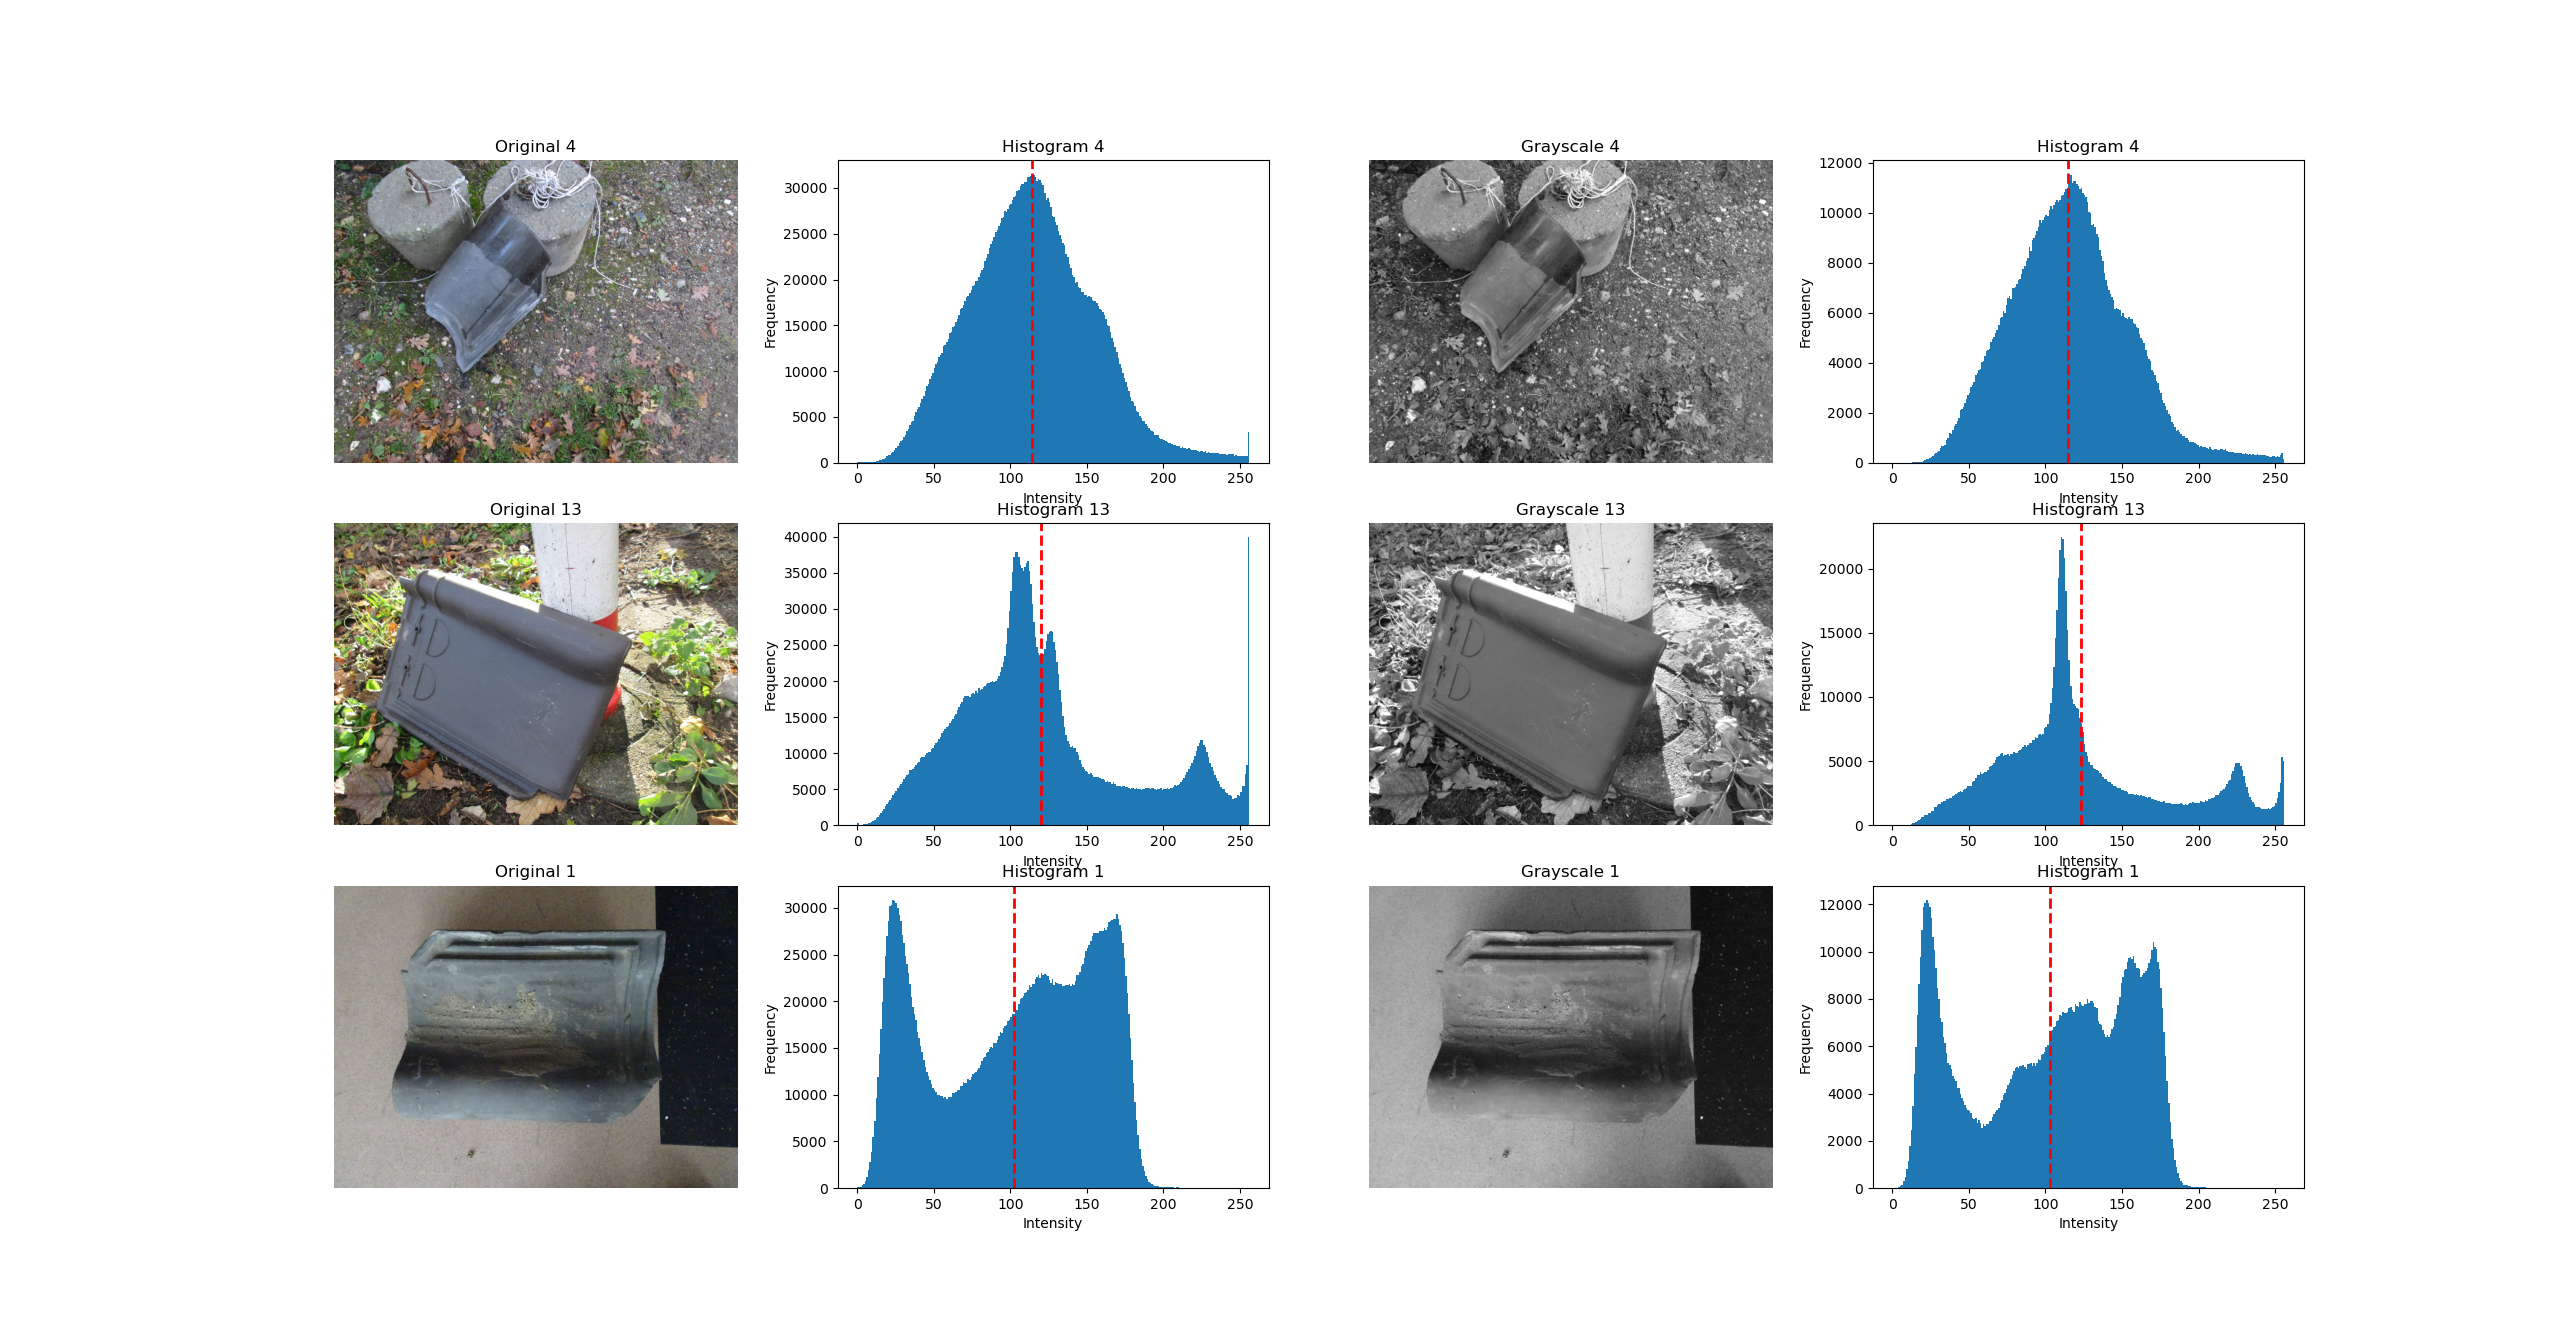
\includegraphics[width=\linewidth]{grayscale_graph_histogram.png}
	\caption{Grayscale of images plot}
	\label{fig:grayscale_graph_histogram} % Label for referencing this figure in the text automatically
\end{figure}

\newpage
\subsection{Applying normalization}
\sidenote[][1cm]{After grayscaling, normalization needs to be applied to normalize contrast. 
Doing this removes some glare or extreme lighting effects caused by the camera lens.}
\begin{figure}[H] % [H] forces the figure to be output where it is defined in the code (it suppresses floating)
	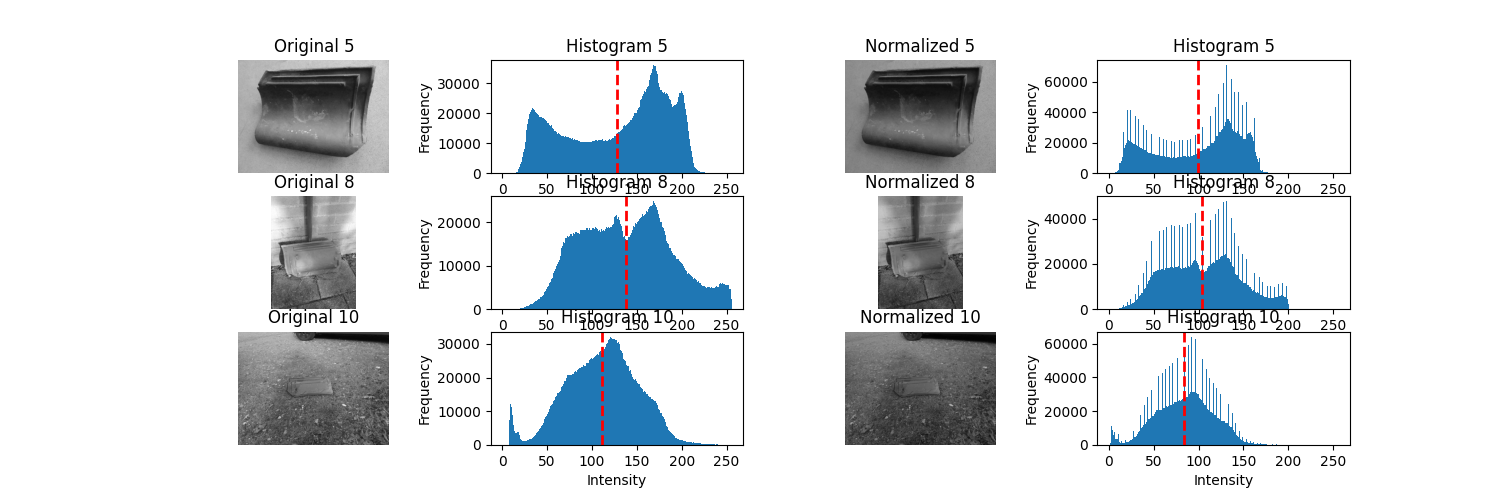
\includegraphics[width=\linewidth]{normalization_conversion_before_after.png}
	\caption{Normalization of images plot}
	\label{fig:normalization_conversion_before_after} % Label for referencing this figure in the text automatically
\end{figure}

% \newpage
\subsection{Applying CLAHE}
\sidenote{Lastly, CLAHE is applied to bring out more details. 
CLAHE does this to dampen some of the higher pixel values and placing them below the average threshold, 
so that details appear more sharp.}
\begin{figure}[H] % [H] forces the figure to be output where it is defined in the code (it suppresses floating)
	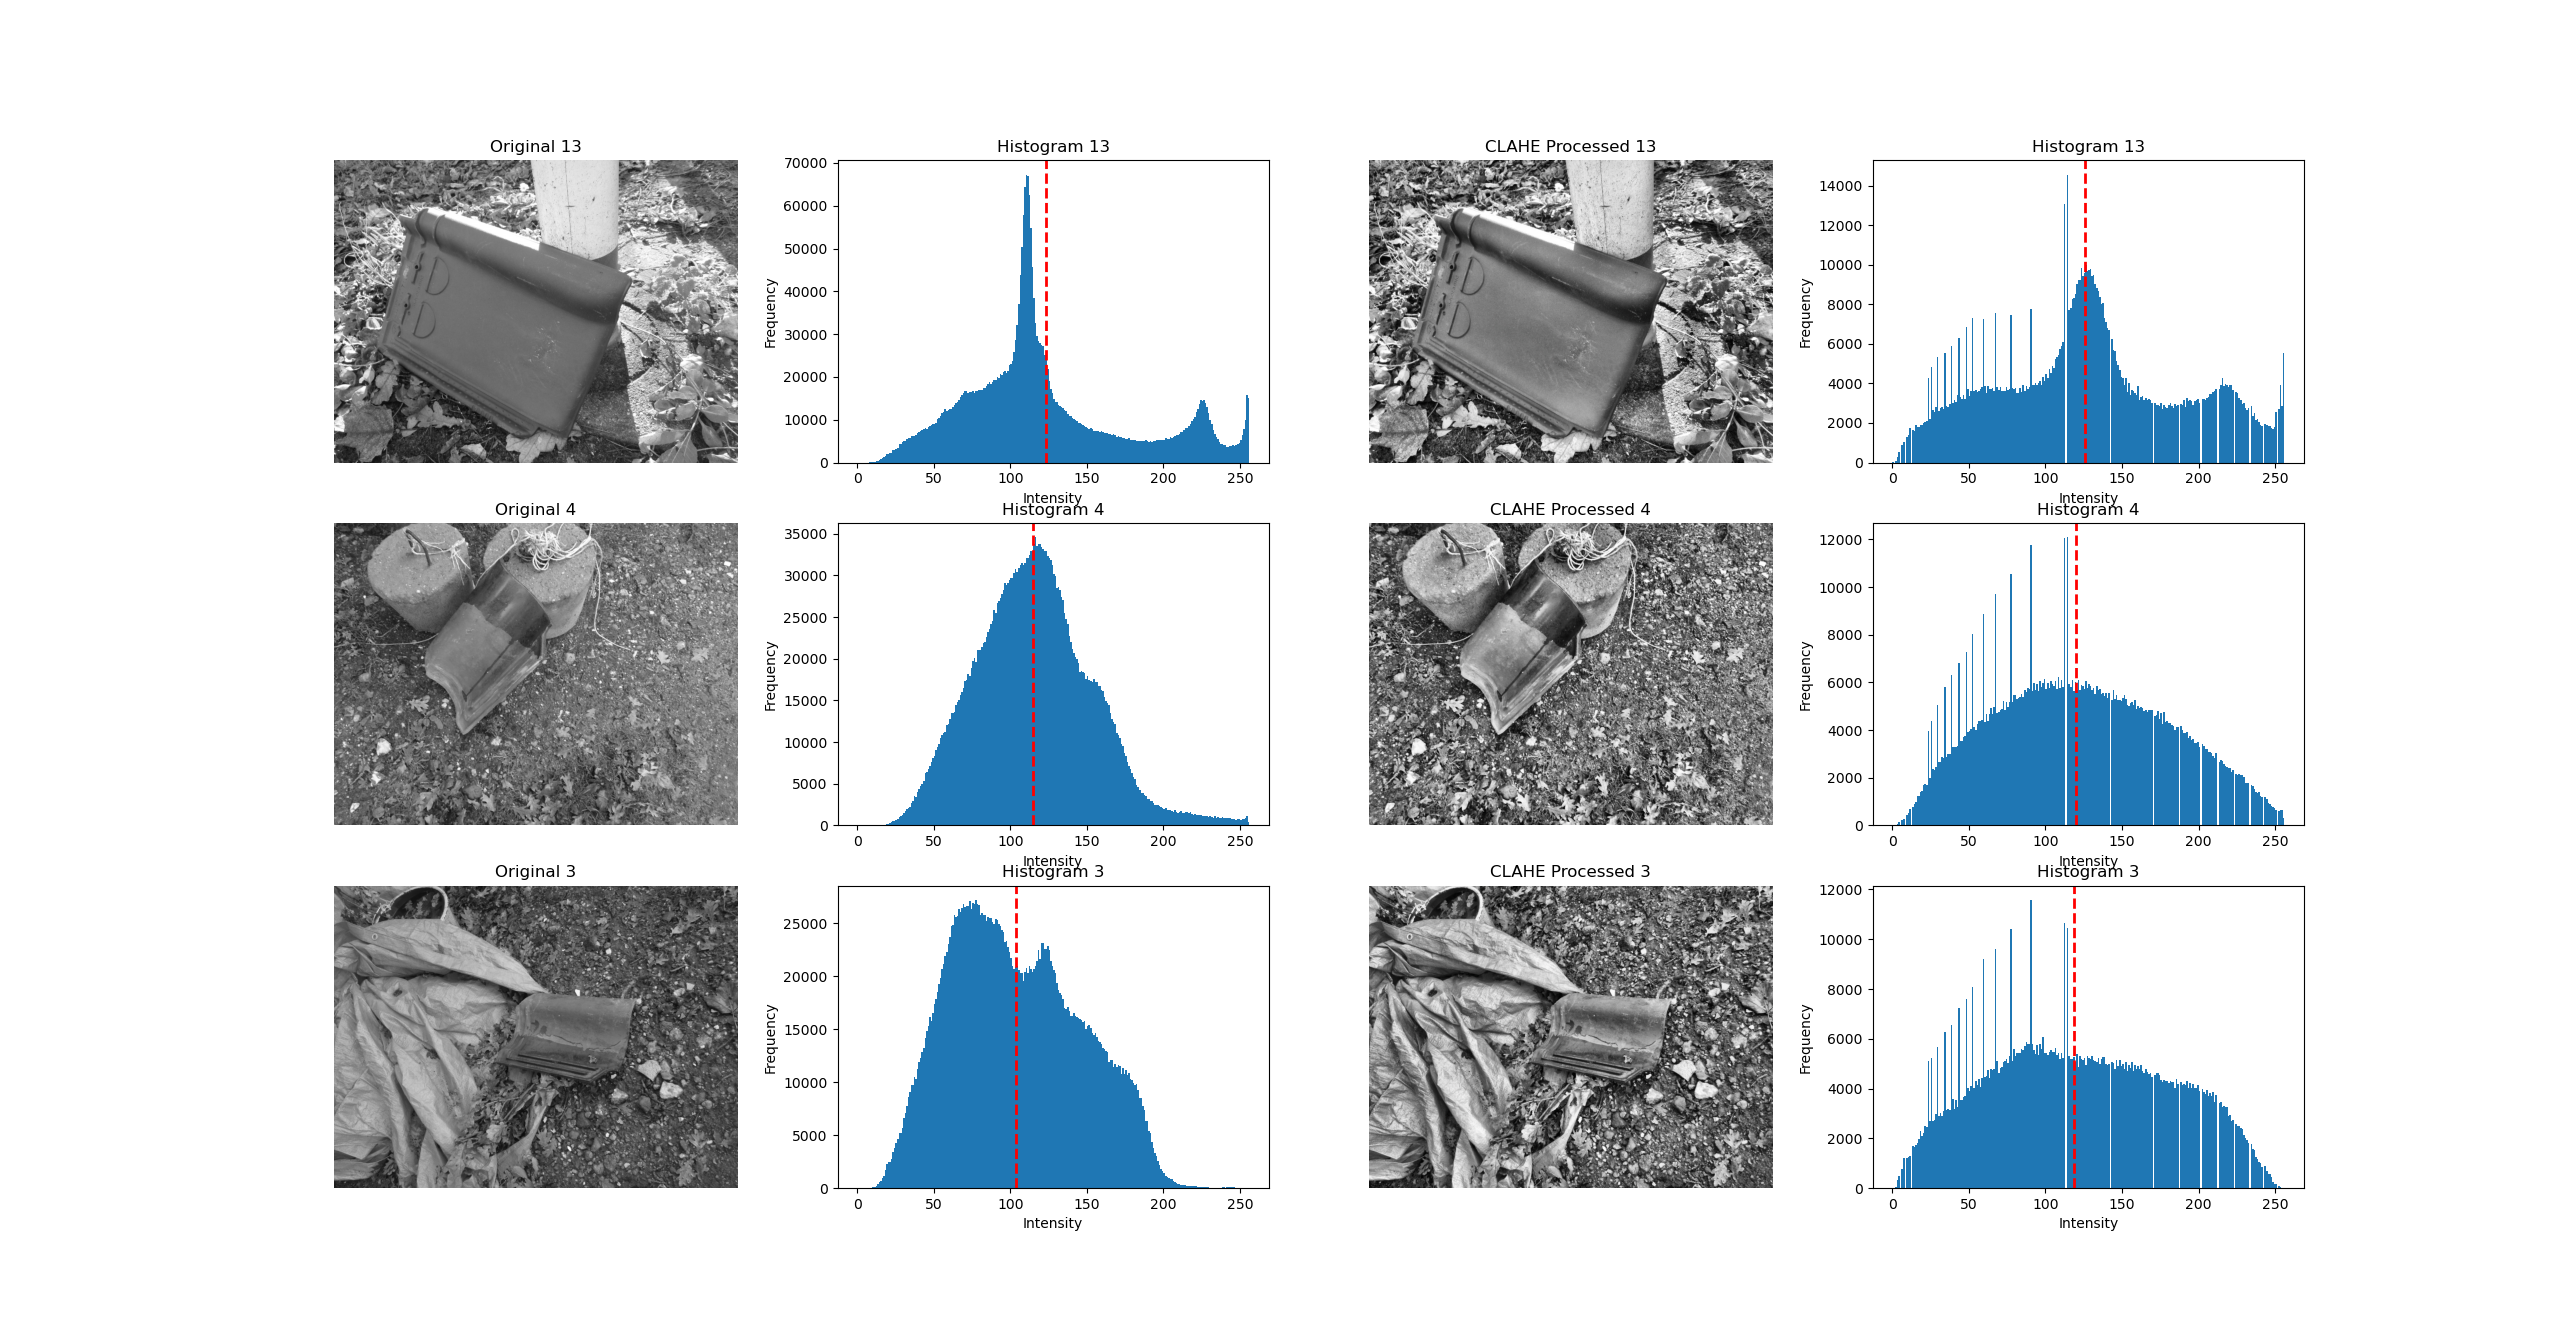
\includegraphics[width=\linewidth]{clahe_graph_histogram.png}
	\caption{CLAHE of images plot}
	\label{fig:clahe_graph_histogram} % Label for referencing this figure in the text automatically
\end{figure}

\newpage
\subsection{Image resizing}
Since most image recognition models require the images in the dataset to be of square format, and images in our dataset were not square, we came up with a technique to make non-square images square. First, we resized images to target resolution (640 by 640).
\begin{marginfigure} % Use the marginfigure environment for figures to be output to the margin
	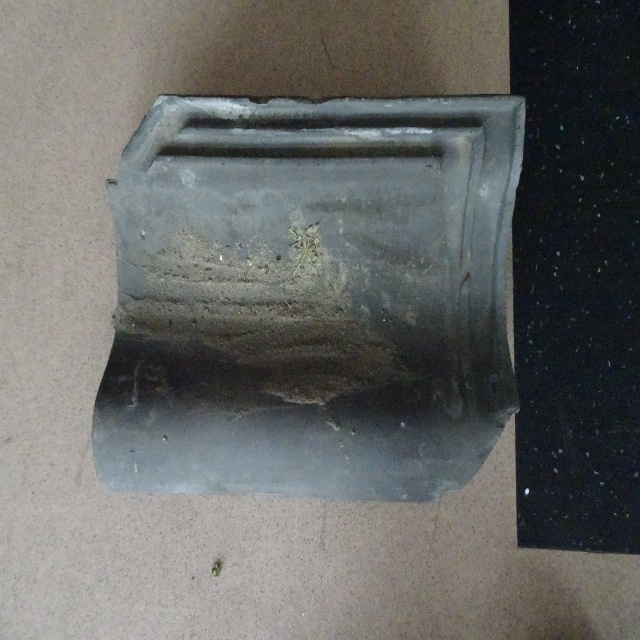
\includegraphics[width=\linewidth]{square_dataset/square0.JPG}
	\caption{An example of resized image that is streched.}
\end{marginfigure}

However, simply resizing images to the target size is not sufficient since images in the dataset are not square. Simply resizing images will make resized images streched, which might be harmful in training the model.

\begin{marginfigure} % Use the marginfigure environment for figures to be output to the margin
	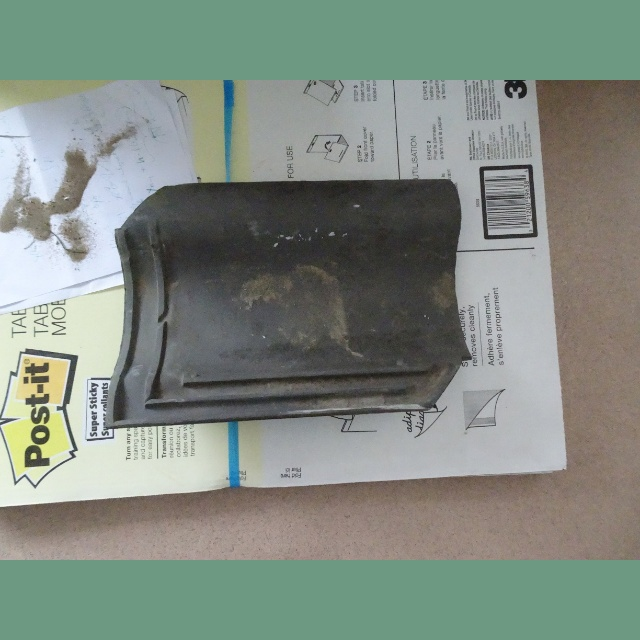
\includegraphics[width=\linewidth]{square_dataset/square1.JPG}
	\caption{An example of horizontal resized image.}
\end{marginfigure}

To convert none square images to square images, we add background to the images. This is done by placing padding with a random color around the image to fill up the blank space required to make it square.
Depending on whether the original image is vertical or horizontal, we add vertical padding or horizontal padding so that the final image becomes square.


\begin{marginfigure} % Use the marginfigure environment for figures to be output to the margin
	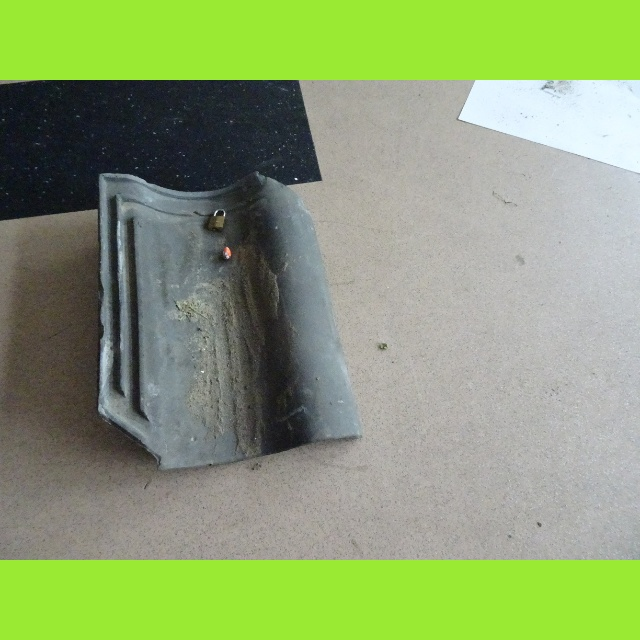
\includegraphics[width=\linewidth]{square_dataset/square2.JPG}
	\caption{Example of resized image.}
\end{marginfigure}

We could simply add a black background to all images but to make sure adding single color background does not add bias to images, we have used random color for the background. 
In the code, the target resolution is 640*640 pixels. This resolution is required by most YOLO-models which could be used as the main algorithm classifying the rooftiles. However, the implemntation of code is genral and can be used for any target resolution. 
To the side are a few examples of images converted to a square aspect ratio.


\begin{marginfigure} % Use the marginfigure environment for figures to be output to the margin
	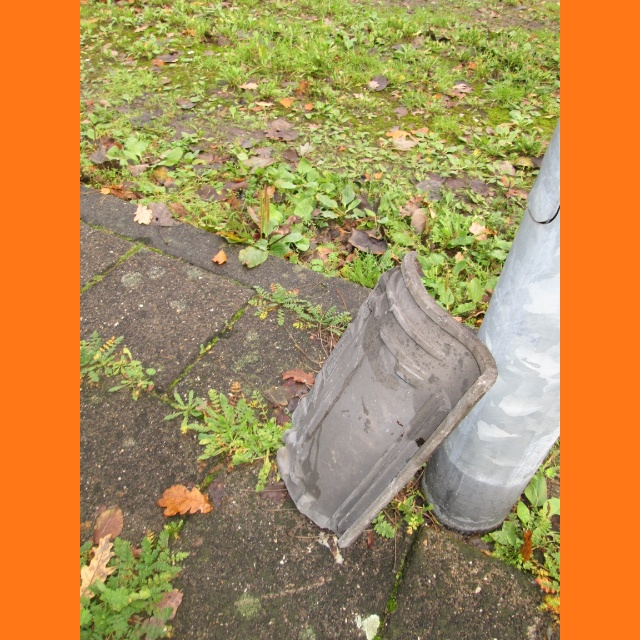
\includegraphics[width=\linewidth]{square_dataset/square3.JPG}
	\caption{Example of vertical image.}
\end{marginfigure}

To explain how the resizing is done, consider the following example: a 1800 by 1200 image that we want to convert to 600 by 600 image (number are chosen for simplicity). To make 1800 by 1200 into 600 by 600 square, first we have to resize it by a factor of 1/3 (it is the minimum of 600/1800 = 1/3 and 600/1200 = 1/2). After resizing the original image by a factor of 1/3, we get to a 600 by 400 image. To make this image square, we need to add 100 pixels of padding to each side of this resized image to get a 600 by 600 image.


% \begin{marginfigure} % Use the marginfigure environment for figures to be output to the margin
% 	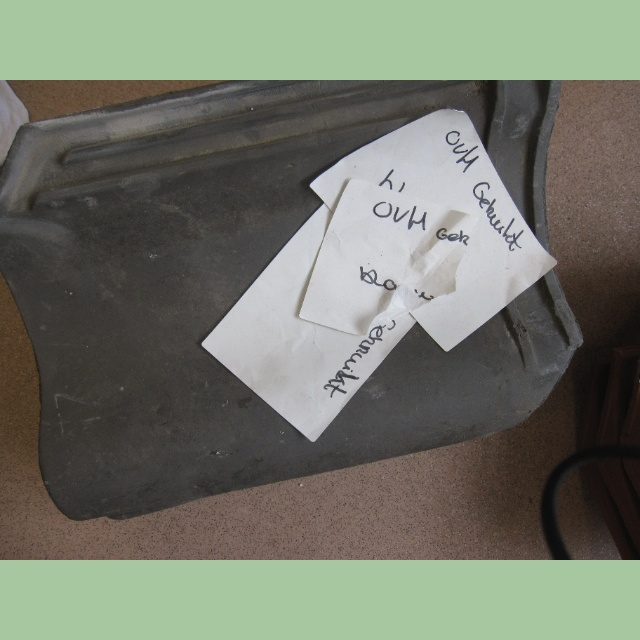
\includegraphics[width=\linewidth]{square_dataset/square5.JPG}
% 	\caption{Square5}
% \end{marginfigure}

\subsection{Data augmentation}
A few augmentation techniques are applied to artificially increase the dataset and training data. 
It's important to realize that this is just done for training and not testing, 
since testing requires the images to be as closely to the real world as possible. 
Below are a few simple techniques which can be applied to any image in the dataset:

\subsubsection{Flipping}
\subsubsection{Rotating}
\subsubsection{Mirroring}
\subsubsection{Zoom}

\subsection{Splitting data}

\subsubsection{Training}
Test

\subsubsection{Testing}

% Lorem ipsum dolor sit amet, consectetur adipiscing elit. Aliquam auctor mi risus, quis tempor libero hendrerit at. Duis hendrerit placerat quam et semper. Nam ultricies metus vehicula arcu viverra, vel ullamcorper justo elementum. Pellentesque vel mi ac lectus cursus posuere et nec ex. Fusce quis mauris egestas lacus commodo venenatis. Ut at arcu lectus. Donec et urna nunc. Morbi eu nisl cursus sapien eleifend tincidunt quis quis est. Donec ut orci ex. Praesent ligula enim, ullamcorper non lorem a, ultrices volutpat dolor. Nullam at imperdiet urna. Pellentesque nec velit eget est pretium.\sidenote{This is a sidenote. This template features a large margin specifically so you can put notes, figures, tables and other things into it as additional material to the main content in the text block.}

% Donec in elit ac ante vestibulum rhoncus. Pellentesque ligula tortor, aliquet malesuada nulla tristique vitae. Aliquam mi sem, varius eu pellentesque et, tristique nec quam. Vestibulum pellentesque in dui et venenatis. Sed malesuada elit pellentesque sapien aliquet porta. In at facilisis diam. Duis id ante tellus.\sidenote[][2cm]{This sidenote has been pushed down the page manually with an optional parameter, otherwise it would be right under the one above.} % This first optional argument to a sidenote is the symbol to use (leave this empty for automatic numbering) and the second is the vertical offset (positive is down, negative is up)

% \subsection{Subsection Title} % Second level section

% In diam libero, vulputate quis accumsan non, auctor in ipsum. Praesent cursus velit eget lacus sodales porta. Proin quis risus ut velit euismod scelerisque ut sed neque. Cras sagittis, dolor ac ullamcorper auctor, tortor dui facilisis diam, at sagittis nisi ipsum a neque. Nullam vel mattis nisi. Ut interdum ut diam at ornare. Nulla ultrices elit justo, vitae tristique massa vulputate sit amet.

% \nonumsidenote{This sidenote isn't numbered in the text or margin. This is useful for notes that apply anywhere on the page instead of one particular place.}Vestibulum erat felis, cursus vitae convallis ac, commodo eu nisi. Nulla facilisi. Mauris dignissim nisi felis, a mollis ex accumsan vel. Suspendisse bibendum vitae nibh in suscipit. Vestibulum et finibus eros. Nulla facilisi. Cras luctus aliquam finibus. In nec justo nec orci malesuada faucibus.

% \subsubsection{Subsubsection Title} % Third level section

% \begin{fullwidth} % Use the whole page width
% 	\textit{This is an example of a full width paragraph\ldots} Curabitur id placerat orci. Vivamus pulvinar augue ac feugiat blandit. Donec in ultricies mi. Nam eu lacus ac augue aliquet consectetur. Praesent dui risus, sollicitudin nec felis ut, posuere ultricies dolor. Sed massa nulla, dignissim eget sem sit amet, eleifend fermentum dui. Phasellus consequat sem vel turpis finibus, a aliquam risus malesuada.
% \end{fullwidth}

% Maecenas consectetur metus at tellus finibus condimentum. Proin arcu lectus, ultrices non tincidunt et, tincidunt ut quam. Integer luctus posuere est, non maximus ante dignissim quis. Nunc a cursus erat. Curabitur suscipit nibh in tincidunt sagittis. Nam malesuada vestibulum quam id gravida. Proin ut dapibus velit. Vestibulum eget quam quis ipsum semper convallis. Duis consectetur nibh ac diam dignissim, id condimentum enim dictum. Nam aliquet ligula eu magna pellentesque, nec sagittis leo lobortis. Aenean tincidunt dignissim egestas. Morbi efficitur risus ante, id tincidunt odio pulvinar vitae.

% \paragraph{Paragraph Title} % Fourth level section

% Lorem ipsum dolor sit amet, consectetur adipiscing elit. Aliquam auctor mi risus, quis tempor libero hendrerit at. Duis hendrerit placerat quam et semper. Nam ultricies metus vehicula arcu viverra, vel ullamcorper justo elementum. Pellentesque vel mi ac lectus cursus posuere et nec ex.

% The section titles below show how multi-line section titles look at the 3 top levels.

% \section[Short version of long section title]{Fusce eleifend porttitor arcu, id accumsan elit pharetra eget} % Use the optional parameter to the \section command to specify a shorter version of the title for the table of contents

% Lorem ipsum dolor sit amet, consectetur adipiscing elit. \nonumsidenote[-2cm]{Section, subsection and subsubsection titles can span multiple lines, as shown here. Make sure to put a shorter version of these long titles in the optional parameter to the section commands so the title output to the table of contents is the short version.}

% \subsection[Short version of long subsection title]{Phasellus sit amet enim efficitur, aliquam nulla id, lacinia mauris viverra libero ac magna}

% Lorem ipsum dolor sit amet, consectetur adipiscing elit.

% \subsubsection{In mi mauris, finibus non faucibus non, imperdiet nec leo. In erat arcu, tincidunt nec aliquam et, volutpat eget}

% Lorem ipsum dolor sit amet, consectetur adipiscing elit.

%----------------------------------------------------------------------------------------
%	FIGURES
%----------------------------------------------------------------------------------------

% \section{Figure Examples}

% This statement automatically references the figure below using its label: Figure \ref{fig:example}.

%------------------------------------------------

% \begin{marginfigure} % Use the marginfigure environment for figures to be output to the margin
% 	
\includegraphics[width=\linewidth]{placeholder.jpg}
% 	\caption{Margin figure caption.}
% \end{marginfigure}

% %------------------------------------------------

% \begin{figure}[H] % [H] forces the figure to be output where it is defined in the code (it suppresses floating)
% 	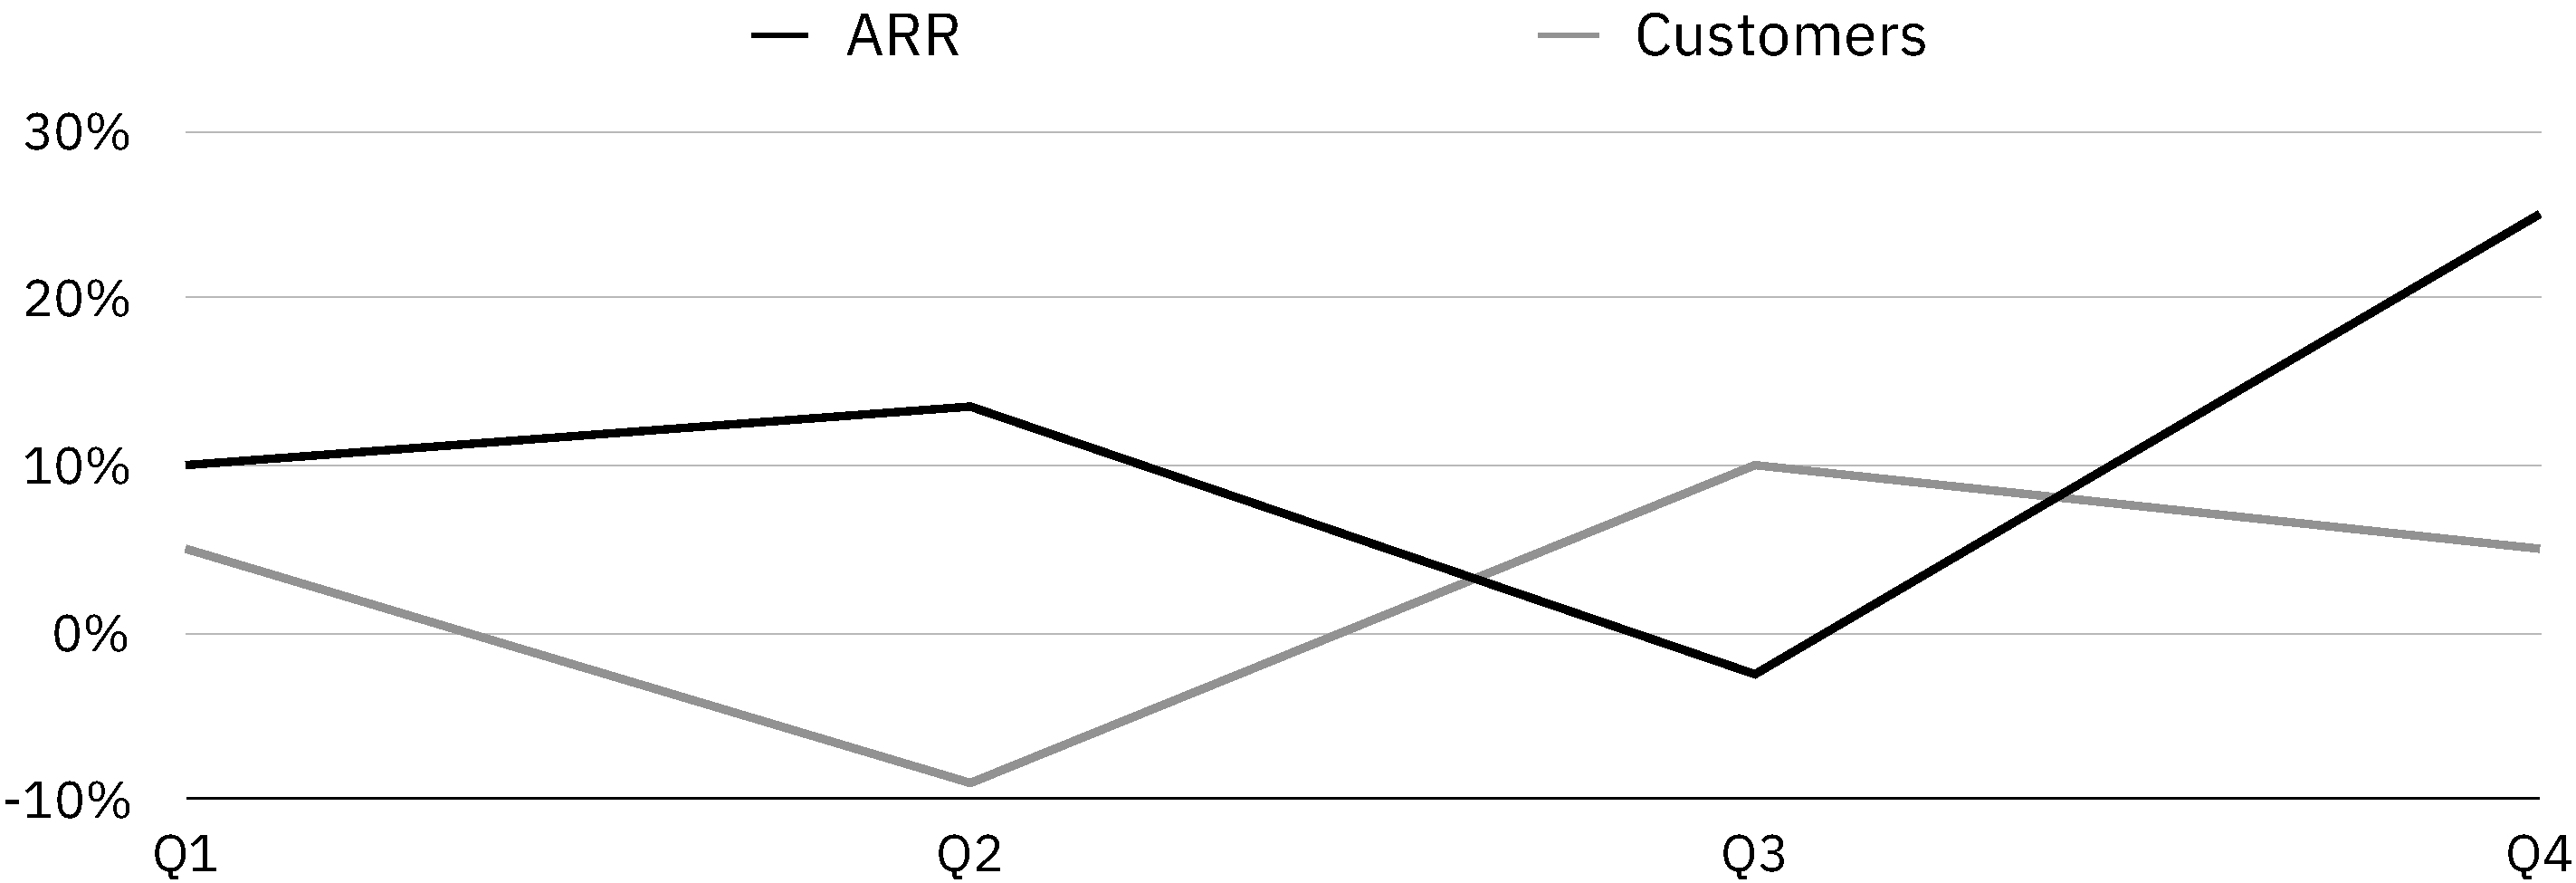
\includegraphics[width=\linewidth]{ARR.pdf}
% 	\caption{Text block figure caption.}
% 	\label{fig:example} % Label for referencing this figure in the text automatically
% \end{figure}

% %------------------------------------------------

% \begin{figure*} % Use the figure* environment for full width figures
% 	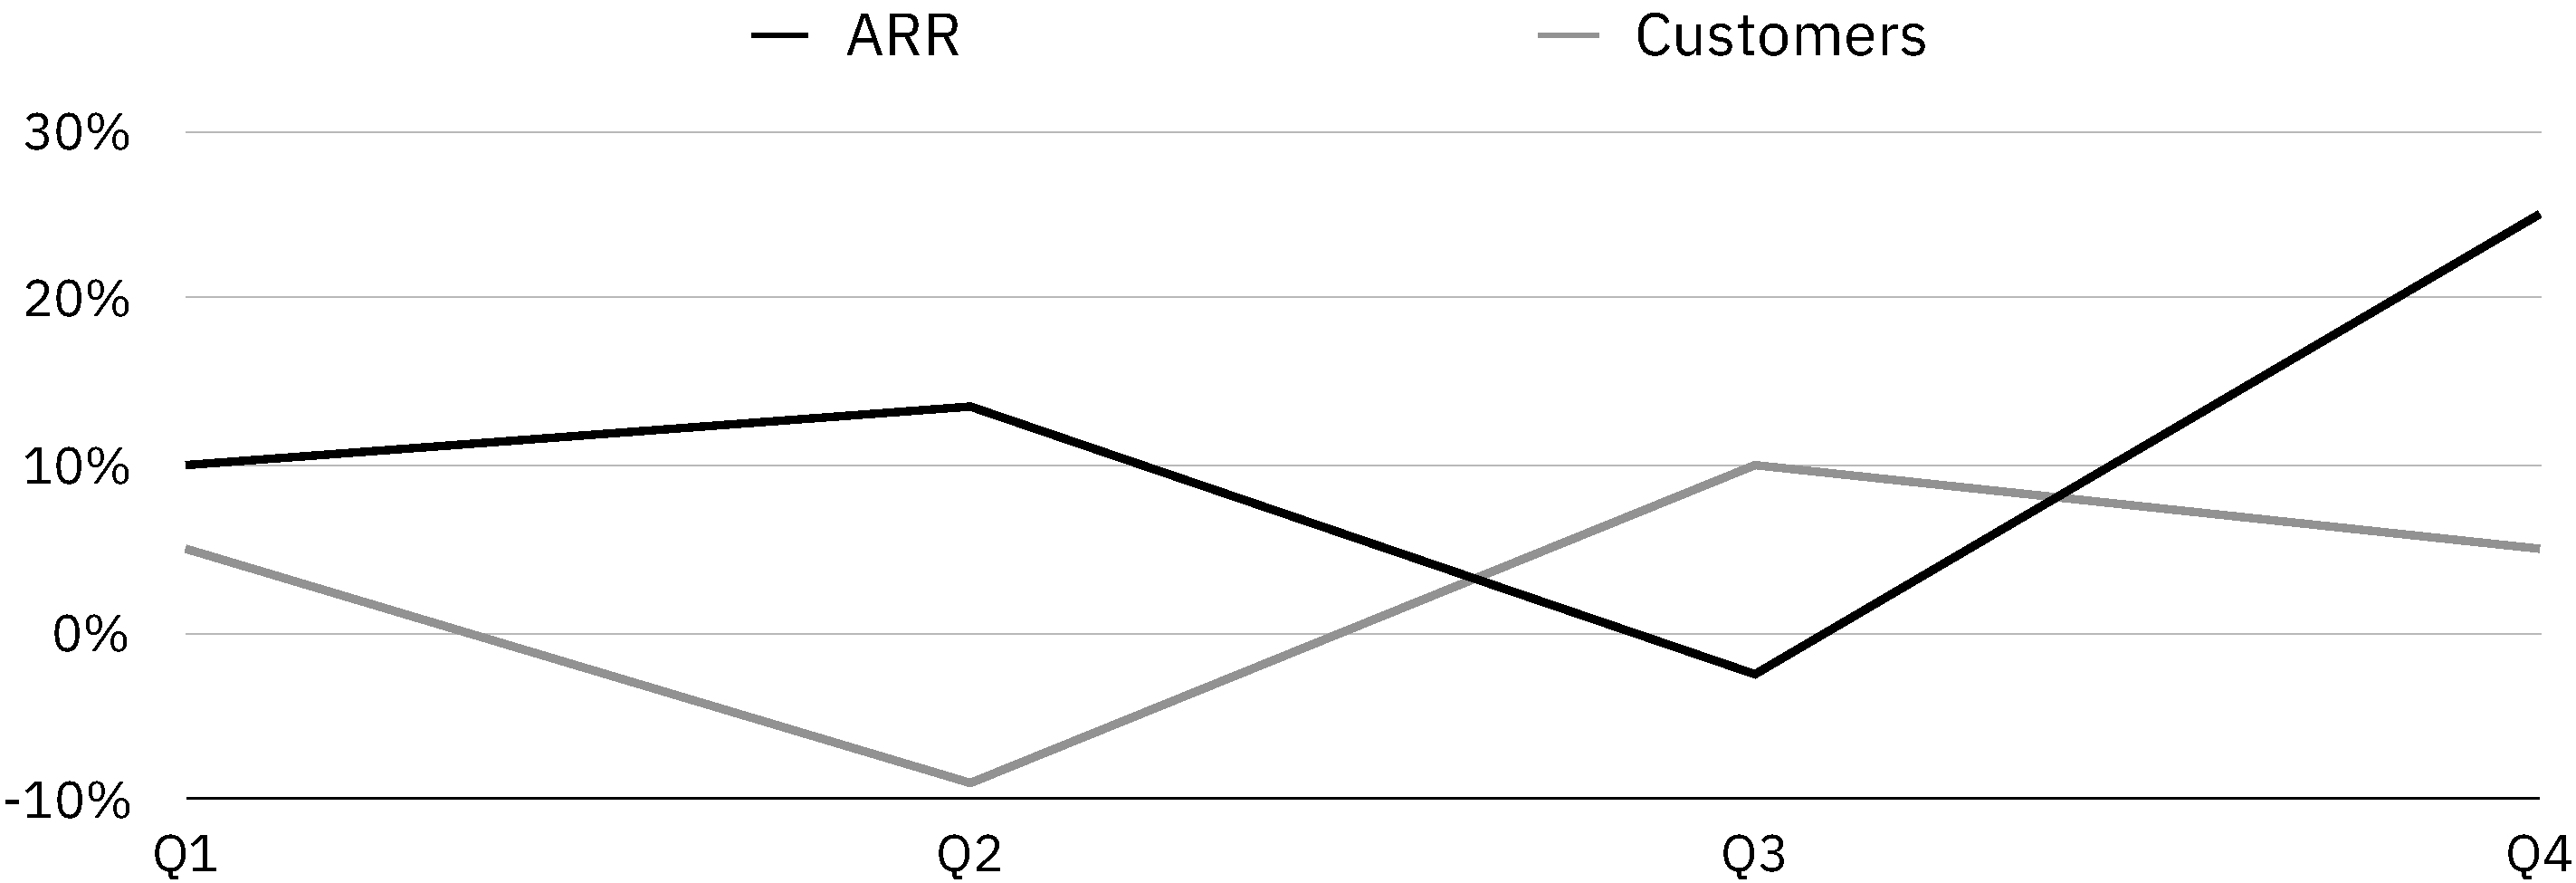
\includegraphics[width=\linewidth]{ARR.pdf}
% 	\caption{Full width figure caption.}
% \end{figure*}

%----------------------------------------------------------------------------------------